\newpage
\section{Static network analysis}

  The bipartite network was created using the users and the words filtered out of stop words and function words. Word list was then additionally limited with Zipf's law in mind: nodes representing $100$ of the most occurring words (not being keywords) and $10\%$ of the words occurring the least were removed from the network (these were with $11$ or less occurrences). Table \ref{tab:filtered_words} shows examples of words that were removed. It is understandable that they would only noise the results.  
  \begin{table}[H]
    \begin{subtable}{0.49\textwidth}
      \centering
      \begin{tabularx}{0.75\textwidth}{|L{1}|L{1}|} \hline
        \rowcolor[gray]{0.8} \textbf{The most used} \\\hline
        guys \\
        question \\
        response \\
        lol \\
        btw \\
        \hline
      \end{tabularx}
      \caption{Some of the most used.}
      \label{tab:filtered_words_top}
    \end{subtable}
    \begin{subtable}{0.49\textwidth}
      \centering
      \begin{tabularx}{0.75\textwidth}{|L{1}|L{1}|} \hline
        \rowcolor[gray]{0.8} \textbf{The least used} \\\hline
        wehre \\
        phenominon \\
        inmate \\
        pacino \\
        more \\
        \hline
      \end{tabularx}
      \caption{Some of the least used.}
      \label{tab:filtered_words_bottom}
    \end{subtable}
    \caption{Selected examples of the most and the least used non-keyword words.}
    \label{tab:filtered_words}
  \end{table}
  
  \subsection{Network simplification}

    Network built using above data was made out of $72,363$ nodes, of which $51,938 (71.77\%$) being users and $20,435 (28.23\%)$ being words, connected by $5,497,840$ edges. This was a massive network in a need of a major simplification. The number of edges was especially important to reduce. I have chosen an edge pruning network simplification, introduced by Zhou \textit{et al.}\cite{ZhouMahlerToivonen2012}. They have proposed a generic framework of network simplification by sharing new methods for pruning the edges while keeping the graph maximally connected. It is important to note that this method is lossy, which means we lose some information from the graph. The method is intended to be used with weighted graphs. In our network, the weights represent the probability that the user have used the word, i.e. the number of times he used this particular word divided by the number of total words he or she wrote. Then, the connectivity would be defined as the maximum probability.
    
    Additional definitions are required to understand the problem. Let \emph{path} $P$ be a set of edges $P = {(u_1, u_2), (u_2, u_3), \ldots (u_{k-1}, u_k)} \in E$. I use the notation $P(u_1 \to u_k)$ to represent the path between $u_1$ and $u_k$ ($u_1$ and $u_k$ being endvertices of $P$).
  
    The problem is parameterised with a \emph{path quality function} $q(P) \to \mathbb{R}^+$. The form of this function is dependent on the type of the graph. In our graph it is the probability that a path exists. We can then assume that the value of any path quality function in this graph is positive, and that a larger value of $q$ indicates better quality.
    
    Given two nodes $u$ and $v$ in a weighted graph, they might be linked by a direct edge or a path, or none when the graph is disconnected. A simple way of quantifying if and how strongly they are connected is to examine the quality of the best path between them\cite{ToivonenMahlerZhou2010}. Thus, the connectivity between two nodes $u, v \in E$ is defined as
    \begin{equation}
      C(u, v; E) = \left\{
      \begin{array}{l l}
        \mbox{max}_{P \subset E: P(u \to v)} q(P) & \quad \text{if such $P$ exists}\\
        -\infty & \quad \text{otherwise.}
      \end{array}
      \right.
    \end{equation}
    A natural measure for the \emph{connectivity} of this graph is then the average connectivity over all pairs of nodes
    \begin{equation}
    C(V, E) = \frac{2}{|V|(|V|-1)} \sum_{u, v\in E, u \neq v} C(u, v; E) \mbox{.}
    \end{equation}
    
    This network was connected so there is no need to calculate the connectivity for each disconnected component and we know that $C(V, E) > 0$.
    
    The goal would to produce a graph $H(V, F)$ that is simplification of graph $G$ and $F \subset E$ such that the \emph{ratio of connectivity} is maximised. A ratio of connectivity is defined as
    \begin{equation}
     rk (V, E, E_R) = \frac{C(V, E \ E_R)}{C(V, E)} \mbox{,}
    \end{equation}
    where $E_R \subset R$ is a set of edges to be removed from the graph and $C(V, E \ E_R)$ is the connectivity of the graph after edges $E_R$ has been removed. The connectivity of the graph obviously cannot be increased while removing edges, thus $rk = 1$ means that the connectivity was left unchanged, $0 < rk < 1$ means that the removal resulted in some loss of connectivity, while $rk = -\infty$ means that the graph has been disconnected.
    
    \begin{algorithm}[H]
      \begin{algorithmic}[1]
        \Procedure{PruneNaively}{$G(V, E)$}
          \State Sort edges $E$ by weights in ascending order.
          \State $F \gets E$
          \State $n \gets (|E| - (|V| - 1))$
          \State $i \gets 1$
          \State $j \gets 1$
          \While{$i \leq n$}
            \If{$C(u, v; F \setminus \{e_j\}$ is not $-\infty$}
              \State $F \gets F \setminus {e_j}$
              \State $i \gets i + 1$
            \EndIf
            \State $j \gets j + 1$
          \EndWhile
          \State Return $H = (V, F)$
        \EndProcedure
      \end{algorithmic}
      \caption{Naive approach.}
      \label{alg:pruning_na}
    \end{algorithm}
    I did not have enough time to conduct \emph{optimal} edge pruning so I have decided to conduct pruning randomly using \emph{naive approach} and see its effects, keeping in mind that $rk$ should be between $0$ and $1$. Algorithm \ref{alg:pruning_na} shows the approach I have selected. It sorts edges by their weights in ascending order first and then iteratively removes edges from the top of the lists when this operation would not cause the graph to be cut. The most important reason why I favoured this approach over the \emph{brute force} (that is not described here) algorithm is that it consists of less steps and is much less time consuming (in fact, it is the quickest)\cite{ZhouMahlerToivonen2012}. I could not use \emph{path simplification} or \emph{combinational approach} because it would remove too much information important in my opinion.
    
    Figure \ref{fig:pruning_effect} shows the effect of the naive approach of pruning. The network has $115$ nodes and $134$ edges. A total of $20$ edges were removed, $19$ of which with a weight of $1$ and $1$ of weight $2$. For that kind of network the results are very good: removal of $\approx 15\%$ edges resulted in only $\approx 4\%$ loss of connectivity. Unfortunately, the average path length has increased from $3.35$ to $5.53$ which is illustrated by the node neighbourhood heat map that was calculated using distance from the node with the greatest degree (the biggest one), with edge weights in mind---the less intense the colour, the more distant the node is.
    \begin{figure}[H]
      \centering        
        \begin{subfigure}[b]{0.50\textwidth}
          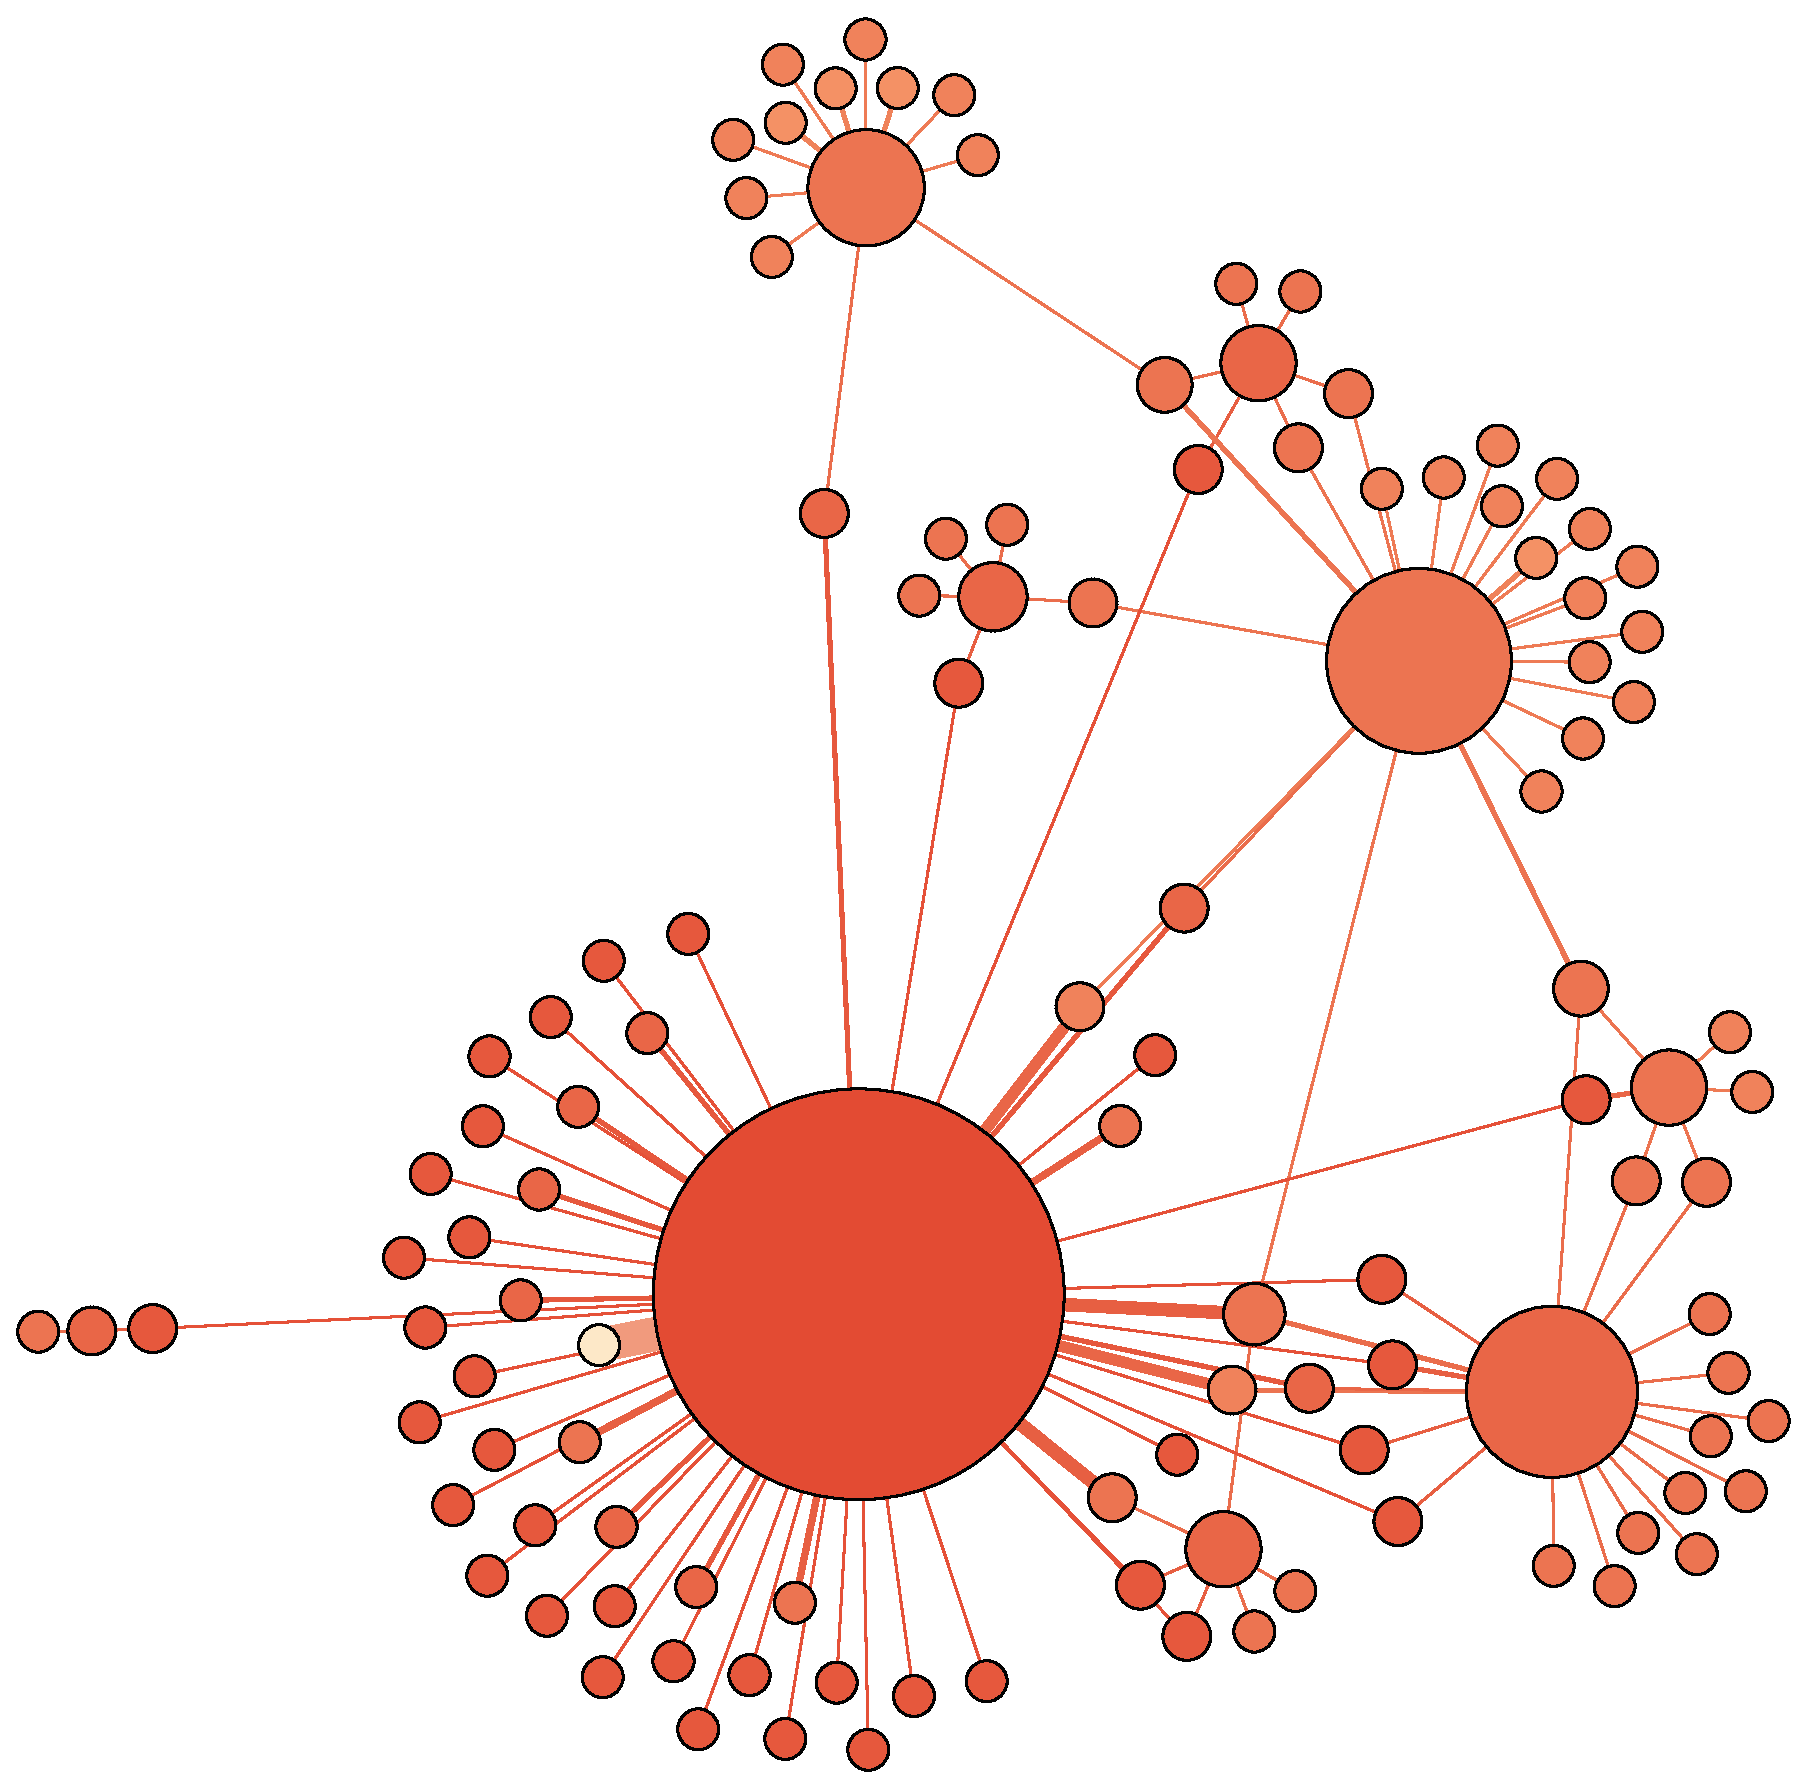
\includegraphics[width=\textwidth]{chapters/03_implementation/prune_1}
          \caption{Before pruning.}
          \label{fig:prune_1}
        \end{subfigure}
        \qquad
        \begin{subfigure}[b]{0.43\textwidth}
          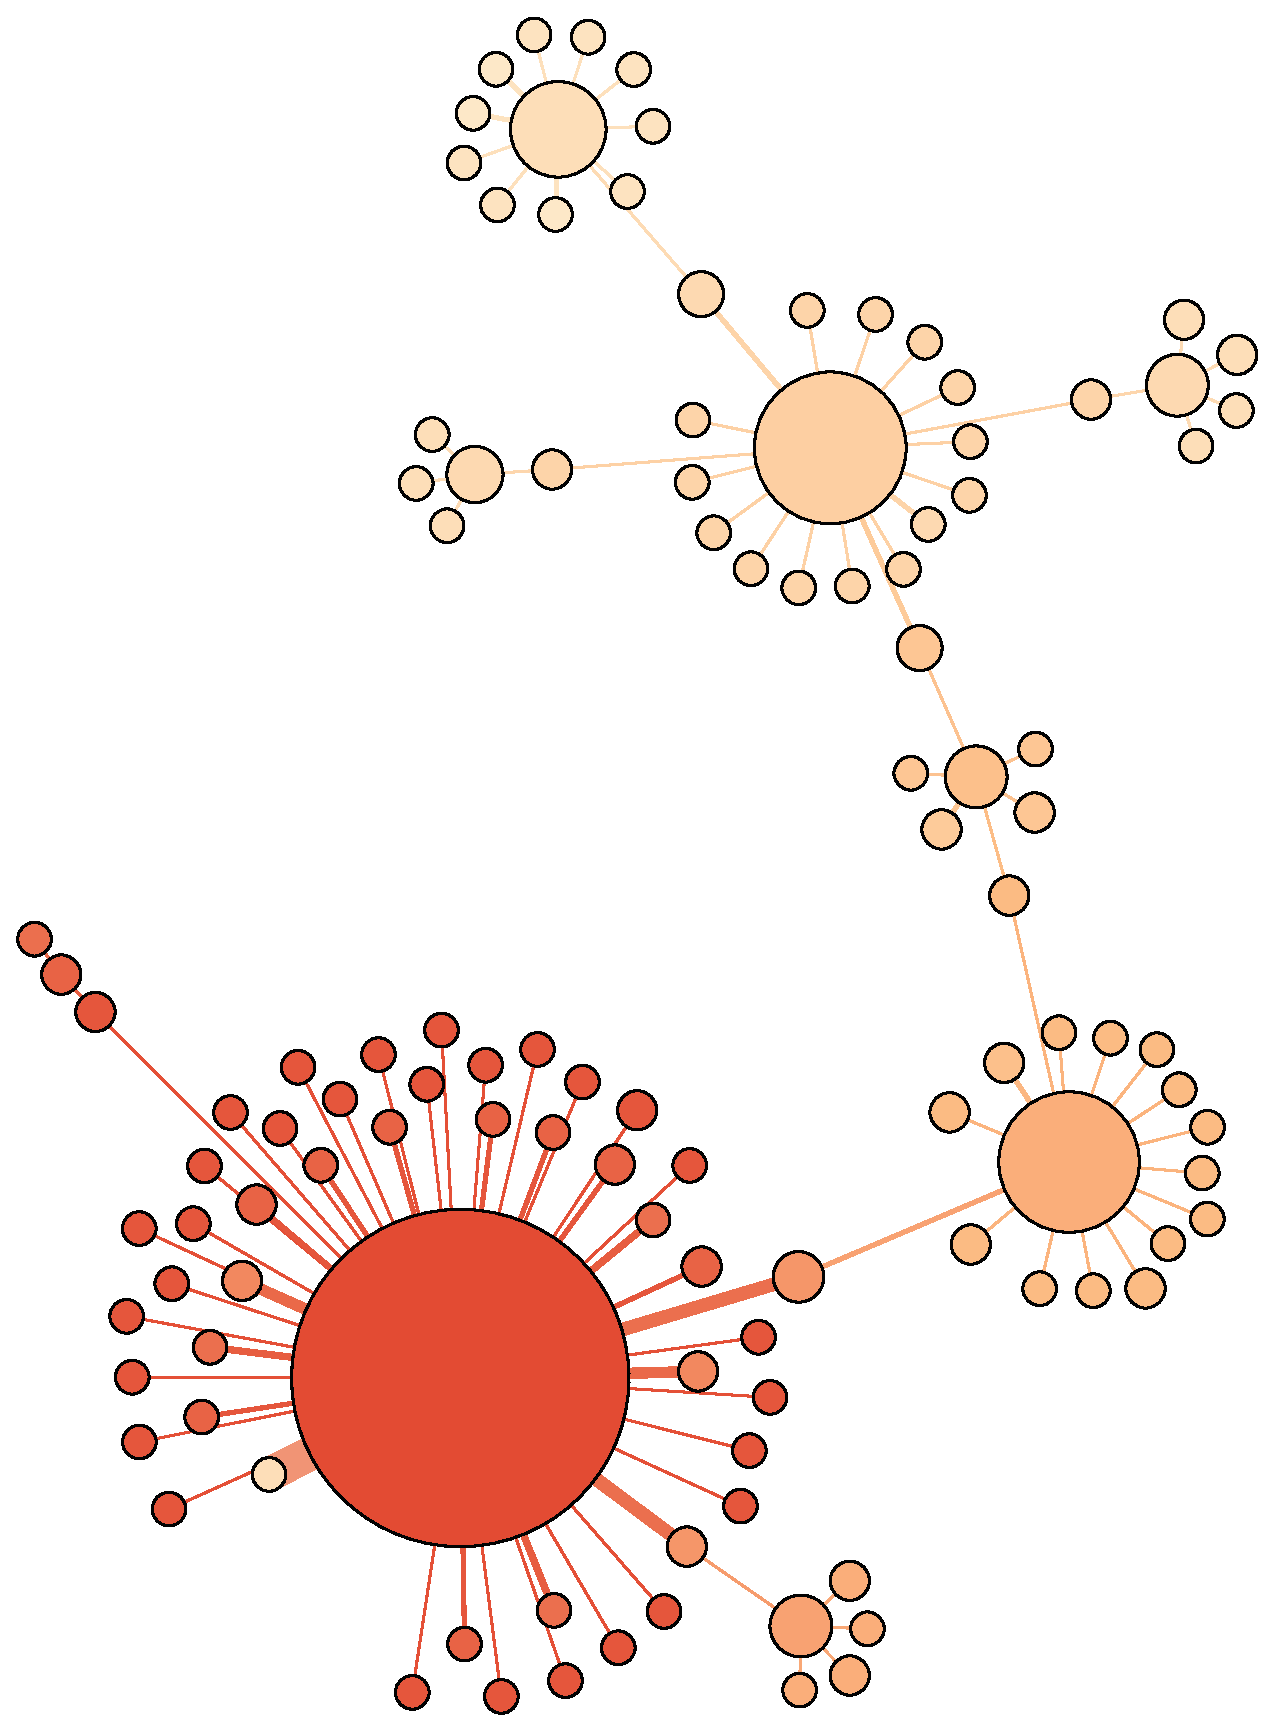
\includegraphics[width=\textwidth]{chapters/03_implementation/prune_2}
          \caption{After pruning.}
          \label{fig:prune_2}
        \end{subfigure}
      \caption{The effect of pruning of example network.}
      \label{fig:pruning_effect}
    \end{figure}
    
    The results of pruning of the whole network are very surprising. It was possible to remove $2,613,126$ edges, which makes a $47.53\%$ of the network! The whole process took around 5 minutes and 12 seconds on my setup: one core of Intel i7 (3740QM) processor and 16GB of RAM. What is even more surprising is the fact that the original connectivity was retained. It is very hard to say why it is the case, but with a high probability I would blame the word extraction process, especially the word splitting pattern which after even so many iterations was apparently not perfect enough.

  \subsection{Network properties}
    The network was then evaluated for its basic properties. They are displayed in table \ref{tab:network_props}. $N$, $M$ and $E$ denote the number of users, words and edges connecting them, respectively. $\langle k \rangle$ and $\langle d \rangle$ are the average user degree and average word degree. The network is made up of one connected component. $\gamma_k$ and $\gamma_d$ are the exponents of the power-law degrees of user degree distribution and word degree distribution respectively. $l_G$ is an average path length, $C$ is the global clustering coefficient and $\langle  C_i \rangle$ is the average local clustering coefficient.
    \begin{table}[H]
      \centering
      \begin{tabularx}{\textwidth}{|L{1}|L{1}|L{1.5}|L{1}|L{0.75}|L{1}|L{0.75}|L{1}|L{1}|L{1}|} \hline
        \rowcolor[gray]{0.8} \textbf{N} & \textbf{M} & \textbf{E} & \textbf{$\langle k \rangle$} & $\gamma_k$ & \textbf{$\langle d \rangle$} & $\gamma_d$ & \textbf{$l_G$} & $C$ & $\langle C_i \rangle$ \\\hline
        $51,938$ & $20,435$ & $2,884,714$ & $55.54$ & $1.63$ & $141.23$ & $1.04$ & $2.68$ & $0.0438$ & $0.0121$ \\\hline
      \end{tabularx}
      \caption{Network properties.}
      \label{tab:network_props}
    \end{table}
    
    Due to the fact that the network is bipartite, we have to check two degree distributions: one for users and one for words they have written. both to follow the power-law
    \begin{equation}
      \begin{split}
        p(k) \sim k^{-\gamma_k} \mbox{,} \\
        p(d) \sim d^{-\gamma_d} \mbox{,}
      \end{split}
    \end{equation}
    with the values of the exponents $\gamma_k$ and $\gamma_d$ shown in table \ref{tab:network_props}.
    
    Figure \ref{fig:degdist_users} shows degree distribution of user nodes. One of the first things that is noticeable while looking at this figure is that the degree distribution for degrees in a range $[1:30]$ is approximately linear and flat. The reason is that there are a lot of users that sign up to this forum with a particular purpose in mind, such as to ask a question or get a recommendation. They create a single topic for their needs and never discuss outside of it and then never return to the forum after they posted their last message. In fact, users having degree $k \leq 30$ and posting only within a single topic represent $69.35\%$ of all the users having such degree. This \emph{in my opinion} explains why the degree distribution $p(k)$ is skewed as much in the degree range $[1:30]$. If we take the other part of the range, i.e. $[31:3950]$, we see that users like that represent only $17.78\%$ of the users from that degree range.
    What is also interesting is rather large number of \emph{hubs}, i.e. users with degree significantly higher than average. Total number of nodes with degree $k \geq 1000$ is $1.24\%$, which makes one user of 80 an important node.
    \begin{figure}[H]
      \centering
      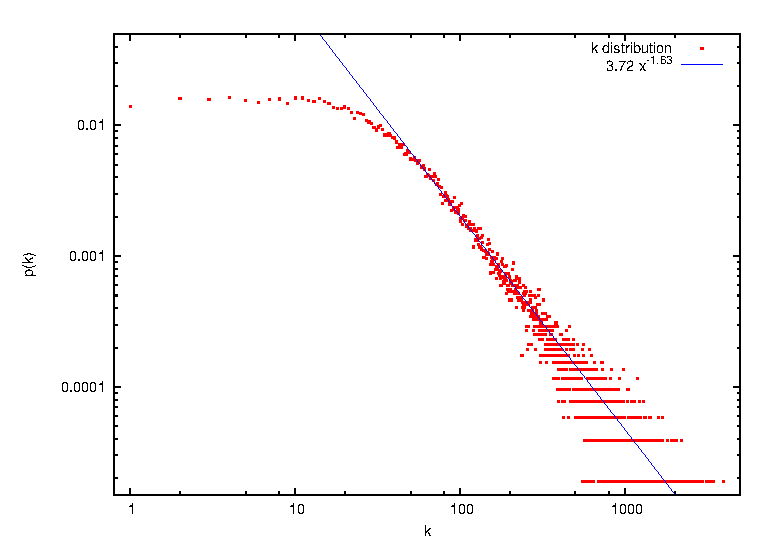
\includegraphics[width=0.76\textwidth]{chapters/03_implementation/degdist_users}
      \caption{Degree distribution of users.}
      \label{fig:degdist_users}
    \end{figure}
    
    The degree distribution of word nodes is shown on figure \ref{fig:degdist_words}. There are no surprises here other than the value of the power-law exponent $\gamma_d$ which is very low, especially where we find the value of this exponent in most real-world scale-free networks to be between $2$ and $3$. I think it is quite safe to assume that if we had no typographical errors in the network and we didn't have to conduct the stemming process, the value would be higher.
    \begin{figure}[H]
      \centering
      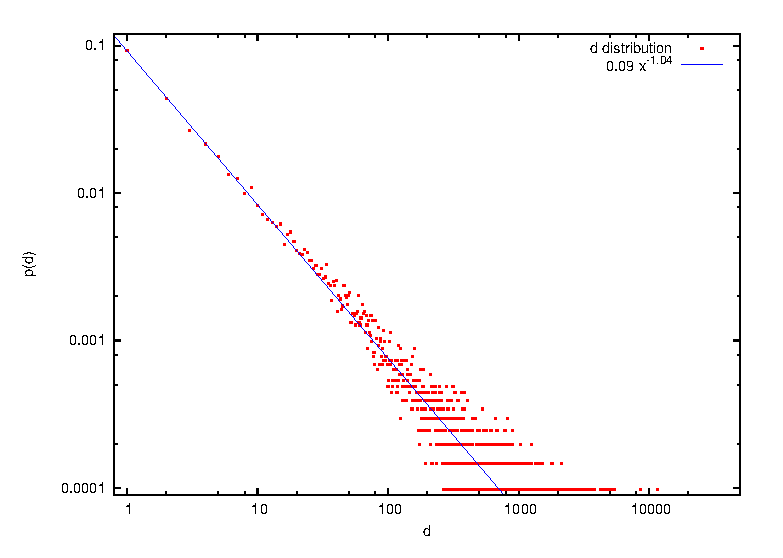
\includegraphics[width=0.76\textwidth]{chapters/03_implementation/degdist_words}
      \caption{Degree distribution of words.}
      \label{fig:degdist_words}
    \end{figure}
